\section{Simple, Discrete Domains}
\subsection{Overview of the Problem}
The first problem is the N-Armed Bandit, a standard problem in reinforcement learning, described by Sutton and Barto (Sutton and Barto, 1998). The N-Armed Bandit problem gets its name from the "one-armed bandit" slot machines in casinos.  The  -armed bandit has more arms, as the name suggests.  The agent must select one of the arms, 'pull' it, and then it receives a variable reward.  The reward is based on a normal distribution that is different for each arm.  The learning problem is to determine which arm has the highest average reward by pulling arms and observing rewards.  The quality of an agent is measured as the percent of times the agent has correctly identified the highest value arm at the end of the learning period.

This problem has only one state and $n$ actions since the agent can choose one of the   arms to pull.  The agent must decide which arm to pull based on the information it has accumulated from previous rewards.  The agent needs to try all arms to get some information about each of them, but should ultimately try to concentrate on the higher-reward arms to find the best one.  The traditional single-agent approach is to keep track of the average reward produced by each arm.  The agent then decides whether to select the arm with the highest reward, or to explore the arms and choose one at random.  The learning parameter, $\epsilon$ , is used to set the probability that a random arm is chosen.  The best arm is chosen with probability $(1-\epsilon)$ .  After the training period, the arm with the highest average reward is the agent’s prediction of the best arm.

TD learning in this domain simplifies to learning $Q(a)$  since there is only one state.  The learning rate, $\alpha$ , is typically set to $1/(n+1)$ where $n$ is the number of times an action has been taken in the past.  This gives the prior estimated value of $Q(a)$ a weight of $n/(n+1)$ and the updated value equals the mean of all observed rewards for action $\alpha$.

Experiments were run using 10-, 100-, and 1000-armed bandits, with qualitatively similar results.  Results shown below are for the 100-armed bandit.

\subsection{Parallel Implementation}
In the parallel implementation for this problem the agents share their information periodically.  The processing is split between periods of learning where each agent operates independently and a sharing period where the information is consolidated from all agents and then shared.  The actual learning and sharing take place on the GPU while the CPU controls the overall process.  The high level division of activities between CPU and GPU is shown in Figure~\ref{fig:seq_diag}.  This diagram shows the basic paradigm I used for the parallel implementation of learning algorithms using the GPU.  It will be updated as the need arises as domains become more complex.

\begin{figure}[hbtp]
\center
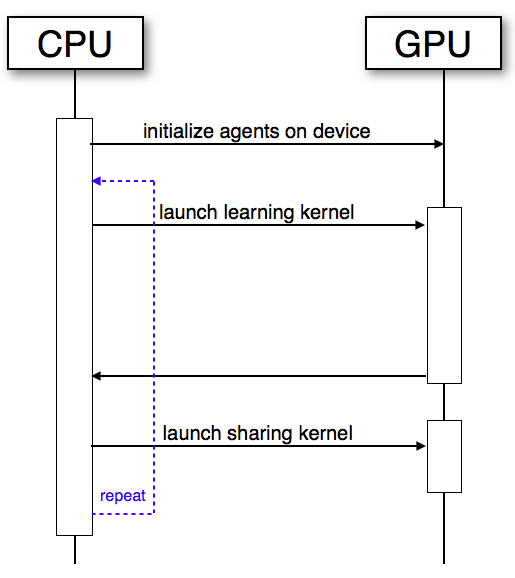
\includegraphics[scale=0.3]{fig01a}
\caption{high-level sequence diagram showing activities on CPU and GPU}
\label{fig:seq_diag}
\end{figure}

\begin{flushleft}

Key learning parameters for the multi-agent parallel approach for the  -Armed Bandit are:

\begin{itemize}
\item
The exploration probability, $\epsilon$ , same as in the single agent algorithm,
\item
the number of parallel agents, and
\item
the frequency of information sharing.
\end{itemize}

\subsection{Sharing and Differentiation}
Each agent keeps track of the number of pulls for each arm and the arm’s average payout.  When sharing occurs an overall count and average is calculated for the block of agents, and then shared back to all agents.  Let $n_i^{[j]}$ be the number of pulls stored by agent $i$ for arm $j$, and $Q_i(j)$ be the value estimated by agent $i$ for arm $j$.  The total values are calculated and each agent is updated based on the following equations for each arm $j$:

\begin{equation}
n_{total}^{[j]}=\sum_in_i^{[j]}
\end{equation}

\begin{equation}
Q_{total}(j)={ {\sum_in_i^{[j]}Q_i(j)} \over {\sum_in_i^{[j]}}}
\end{equation}

For each agent $i$:

\begin{equation}
Q_i(j) \gets Q_{total}(j)
\end{equation}

\begin{equation}
n_i^{[j]} = n_{total}^{[j]}/\mbox{\it number-of-agents} \label{num_pulls}
\end{equation}

Note that in equation \eqref{num_pulls} the number of pulls stored by each agent after sharing is their share of the total number of pulls, not the total number of pulls for the entire block.  This gives less weight to the averages stored by the agent and allows those values to change more dramatically after sharing has occurred.  It also means that the sum of the number of pulls across all agents is equal to the actual total number of pulls.  This is useful when re-calculating the total values at future sharing points.  The result is that some agent's will have their average value for the best arm go down due to the random nature of rewards, perhaps causing another arm to become the best for that agent.  This has the ultimately beneficial effect of causing agents to explore other arms with high average values.

The next time sharing occurs, the block average is recalculated and quality is improved for all agents.  This gives the agents a periodic burst in learning quality at the point of sharing.  The quality may drop between sharing points as the agent’s own values are allowed to vary.  At each sharing point the quality of each agent is restored and actually improves based on the combined information.

\subsection{Results}
Experiments were run with a number of agent differentiation strategies:
\begin{itemize}
\item
partitioning the arms among the agents so when an agent was exploring it would only explore its assigned arm,
\item
random bias given to each agent used when choosing the best arm to pull,
\item
giving some agents in a group a high epsilon value so they would explore with a much greater probability than other agents, and
\item
assigning some agents to randomly choose between the top 2 or top 4 arms when selecting the best arm instead of choosing the actual best arm.
\end{itemize}

There was no dramatic improvement in learning quality from these strategies.  For some, a small improvement in learning quality was more than offset by the increased processing time to implement the more complex logic, resulting in poorer learning as a function of learning time.

Experiments were run for 10-, 100-, and 1000-armed bandits using a single agent and groups of from 4 to 8,192 parallel agents.

The results are broken down into two components to gain a better understanding of the cost and benefits of parallelization.  The first component is learning quality as a function of the number agent-time steps.  An agent time-step is one interaction between an agent and its domain, which equates to one cycle of the learning process executed by one agent.  This will measure the “parallelization penalty” which is the expected reduction in learning quality when a fixed number of agent-time steps are spread over multiple parallel agents, as compared to a single agent operating for all of the time steps.  The penalty occurs because the parallel agents operate independently and only periodically share partial information about their experience.  The single agent is expected to have better learning results, when measured on this basis, since it has complete information available at every time step.

Offsetting the parallel penalty is the speed-up in real time of the parallel implementation.  A fixed number of agent-time steps can run faster if they are executed in parallel, so for a fixed learning period, the parallel approach can execute more agent-time steps than the single agent approach.

The first experiment is for a fixed number of agent-time steps.  Learning is run for the fixed number of agent-time steps and then repeated for 1,024 trials.  Learning quality is calculated as the fraction of the 1,024 trials where the agent correctly identified the bandit with the highest expected payout, which can be determined by inspection.  Measuring learning as a function of agent-time steps gives an understanding of the algorithmic ‘parallel penalty’ from splitting up a fixed number of actions over parallel agents. The results for the 100-armed bandit are shown in Figure~\ref{fig:bandit_steps}.  Learning quality on the y-axis is measured by the probability of correctly identifying the best arm over 1,024 trials.  The blue line with circles is the result for a single agent running on the CPU and the other lines are for different numbers of parallel agents.

\end{flushleft}
\begin{figure}[hbtp]
\center
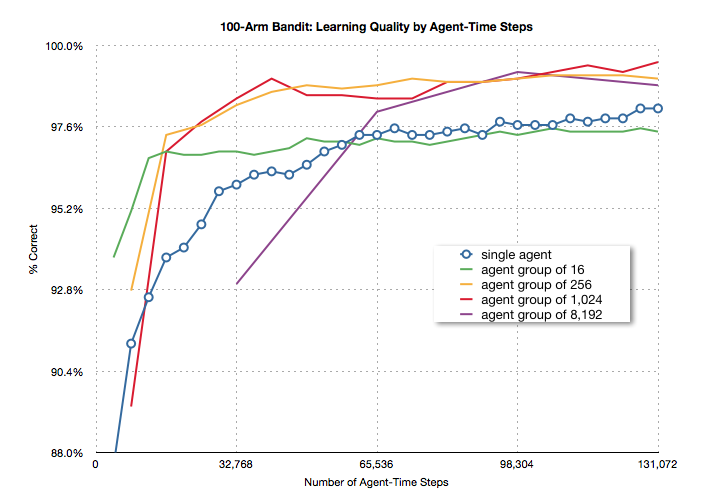
\includegraphics[scale=0.5]{fig02a}
\caption{Learning quality by agent-time steps}
\label{fig:bandit_steps}
\end{figure}

\begin{flushleft}


The results are interesting as there is no clear penalty for the parallel approach, except for agent groups of 16.  When parallel agents numbered 256 or more the parallel implementation actually produced higher quality using a fixed number of agent-time steps.  The difference appears to diminish for extremely large groups as the learning quality drops for 8,192 agents.  The multi-agent advantage is likely coming from more effective exploration due to the lack of complete information.  Each agent in the group makes an independent choice of best arm and the next action to take based on limited information, or perhaps some new unique information it has uncovered but not yet shared, leading to beneficial exploration of the state space.

The next step is to measure learning quality as a function of learning time.  Learning time is the real elapsed time the agent spends interacting with the environment, updating its internal state, and sharing information in the case of parallel agents.  The timing values are for a single learning trial run on the CPU for a single agent, and on the GPU for parallel agents. For parallel runs, the number of time-steps is determined so that the parallel agents took at least as much time as the single agent run for 131,072 time steps.  To get credible quality measurements the results were averaged over 1024 trials for both single agent and parallel agent runs.  Learning quality as a function of learning time is shown in Figure~\ref{fig:bandit_time}.  For the smallest numbers of parallel agents, groups of 16, the parallel implementation on the GPU did poorly compared to the single agent CPU run.  Since the time values were for a single trial, there were only 4 or 16 threads running concurrently on the GPU.  Given the complexity of the calculations and the need to frequently synchronize threads to share information, the poor results are not surprising.  For the larger numbers of parallel agents, with hundreds or thousands of threads, the parallel GPU results clearly surpass the single agent CPU results when learning quality was measured as a function of learning time.

%\end{flushleft}
%\center
%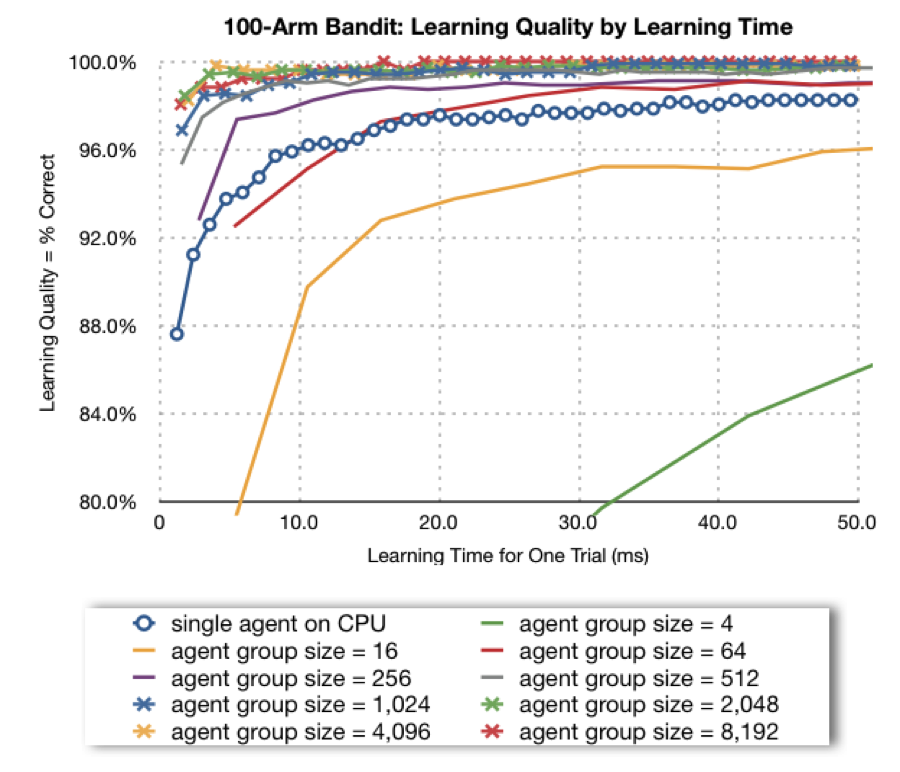
\includegraphics[scale=0.8]{fig04}
%\begin{flushleft}

\end{flushleft}

\begin{figure}[hbtp]
\center
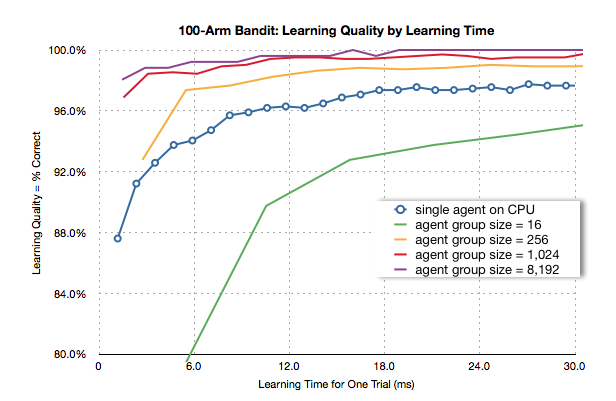
\includegraphics[scale=0.5]{fig03a}
\caption{Learning quality as a function of learning time}
\label{fig:bandit_time}
\end{figure}

\begin{flushleft}


%\end{flushleft}
%\center
%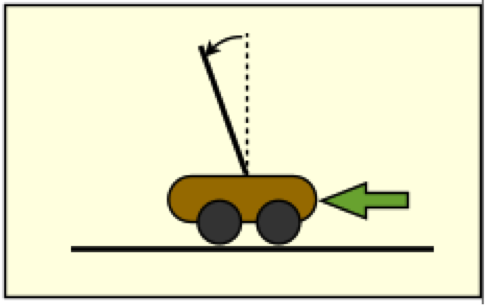
\includegraphics[scale=0.8]{fig06}
%\begin{flushleft}



In summary, the massively parallel approach to the N-armed Bandit problem shows the surprising result that there is no parallel penalty for agent groups of size 64 or larger (Figure~\ref{fig:bandit_steps}).  Splitting a fixed number of agent-state interactions across parallel agents can actually improve the learning quality through more effective exploration.  The parallel results improved further when learning quality is measured as a function of learning time (Figure~\ref{fig:bandit_time}) as the raw speed improvement provided by the GPU allow more agent-time steps to be executed with greater speed in parallel.
